\cleardoublepage

\chapter{Hypothesis and objectives}
\label{sec:problematic}

\cleanchapterquote{Le fait de rêver est sans doute une des données, plus nombreuses qu'on ne le pense, qui, mieux encore que le soleil ou la pluie, placent les hommes de tout climat, de toute époque et de toute condition devant des problèmes identiques.\endnote{Free translation to English: \q{Dreaming is undoubtedly one of the phenomenon, which, better than the sun or the rain, places men of any climate, of any time and any condition in front of identical problems} ---Roger Caillois. L'incertitude qui vient du rêve. 1956}}{Roger Caillois}{L'incertitude qui vient du rêve. 1956}

\section{Unresolved issues}
\label{sec:problematic:unresolved}

From this review of the scientific literature on dreaming, it appears that many questions on the nature, function, and neurophysiological correlates of dreaming remain open, some of which are reported below.

\textbf{Phenomenology of dreaming}
\begin{my_list_item}
    \item Do we dream during the whole night? If not, when do we dream during the night and for how long?
	\item Which factors influence the (dis-)continuity between waking and dreaming?
	% \item Why is there a preferential incorporation of certain waking experiences into dreams?
	\item What are the neurophysiological correlates of dream content? And can we explain the phenomenological content of dream content based on these correlates ?
	\item To what extent lucid dreaming resemble or differ from non-lucid dreaming?
	\item To what extent dreaming resemble or differ from other forms of spontaneous thoughts such as mind-wandering and daydreaming?
\end{my_list_item}

\textbf{Dream recall}
\begin{my_list_item}
	\item Why are there such intra- and inter-individual differences in dream recall frequency?
	\item What are the neurophysiological correlates of dream recall?
    \item Why more dream reports follow awakening from REM sleep than from NREM sleep? Does that mean that the actual \emph{production} of dreams is higher during REM sleep than NREM sleep, or rather than the \emph{recall} of dreams is better following REM sleep?
	\item More broadly, does failure to recall dream upon awakening mean that the sleeper was not dreaming before awakening? Or does this reflect a failure to encode dream content into memory, for example caused by sleep inertia or interference mechanisms?
\end{my_list_item}

\textbf{Function of dreaming}
\begin{my_list_item}
	\item Do dreaming serves an adaptive function \emph{per se}? If so, do they need to reach consciousness and be remembered in order to be functional? Or do they need to be worked, or interpreted as believed by many?
\end{my_list_item}

The present thesis aims at contributing to the ongoing effort to solve these questions, by addressing, in parallel and with different paradigms, several aspects of dreaming. First, we investigated the mechanisms of dream recall by comparing the cerebral and behavioral functioning of high and low dream recallers (HR and LR, respectively). In Study 1 (section \ref{sec:problematic:arousals}), we used EEG recordings to compare the sleep macro- and micro-structure of HR and LR, as well as their brain responses to stimuli during sleep. In Study 2 (section \ref{sec:problematic:inertia}), we compared the cognitive performances and brain functional connectivity of HR and LR during sleep inertia using an EEG-fMRI paradigm. In addition with studying the brain and cognitive alterations during sleep inertia (part 1), our study is the first to experimentally test the hypothesis of a differential sleep inertia between HR and LR (part 2). In Study 3 (section \ref{sec:problematic:dmn-crea}), we further analyzed the data of this EEG-fMRI study to specifically compare the global default mode network functional connectivity in HR and LR, regardless of the effect of sleep inertia. At the same time, we measured, and compared between HR and LR, several cognitive and personality variables. In Study 4 (section \ref{sec:problematic:survey}), we took advantage of the considerable number of responses obtained in the online recruitment survey of this EEG-fMRI study to collect epidemiological data on dream and sleep habits of a large sample of French college students. In Study 5 (section \ref{sec:problematic:wle}), we used dream questionnaires to improve our understanding of the filter that dreaming applies to the waking life memories, and at the same time try to decipher the possible functions of dreaming. Finally, in Study 6 (section \ref{sec:problematic:software}), we leveraged our expertise in sleep analysis to develop a free and open-source software dedicated to the reading, scoring and analysis of sleep data.

\section{Study 1. DRF and intra-sleep awakening: brain mechanisms and functional properties}
\label{sec:problematic:arousals}

We have seen in section \ref{sec:dream-recall:param} that HR tend to have longer awakenings than LR during sleep (2 vs 1 min on average), and consequently a longer duration of intra-sleep wakefulness (30 vs 15 min on average in a full night of polysomnographic-recorded sleep), without any other differences in the duration and proportion of sleep stages \citep{eichenlaub_brain_2014}. These findings support the arousal-retrieval model which states that nocturnal awakenings are necessary to encode dreams into long-term memory. However, if awakenings are crucial for dream recall as these findings seems to suggest, one may ask if there is a minimum duration of awakenings to allow for the successful encoding of dreams into long-term memory, and if so, if this duration varies depending on the pre-awakening sleep stage. This issue was not directly addressed by \citet{koulack_dream_1976}, who merely stated that arousal have to be of \q{sufficient duration to permit consolidation of the dream experience in a form that is accessible in the waking state}.

Consequently, we decided to experimentally test this issue by re-analyzing the data of \citet{eichenlaub_brain_2014} (see section \ref{sec:dream-recall:param:neuro}) in order to score arousals. Arousals correspond to brief and phasic EEG frequency shifts lasting typically between 3 and 15 seconds, and scored independently of the sleep stages (see section \ref{sec:dream-research:sleep:awa-arousal}). To our knowledge, the relationship between DRF and arousals has never been been investigated. In addition with the scoring of arousals, we performed a close comparison of sleep microstructure of HR and LR, in order to extent our knowledge of the influence of sleep parameters on DRF. This analysis included spindles, K-complexes, rapid eye movements and muscle twitches, which were scored either visually or automatically using dedicated algorithms. We also re-examined the data to see whether the longer awakening duration found in HR was limited to a specific sleep stages (e.g. longer nocturnal awakenings following periods of REM sleep), or was present in all sleep stages.

Second, we took the opportunity of the arousals scoring to address another issue, which is related to the finding of differential brain reactivity to auditory stimuli in high and low dream recallers (see section \ref{sec:dream-recall:param:neuro}). As a reminder, \citet{eichenlaub_brain_2014} found that the amplitude of the attention-orienting brain response (P3a) to first names was higher in HR than in LR during both sleep and wakefulness (Fig \ref{fig:intro:jbe-summary}A). These findings, along with the longer intra-sleep wakefulness in high recallers, suggest that there might be a causal link between neurophysiological responses to auditory stimuli and intra-sleep wakefulness during sleep. For instance, the amplitude of brain responses to auditory stimuli could be predictive of subsequent awakening or arousal reactions. Consequently, HR, who have larger brain responses to auditory stimuli, would have in turn more or longer awakenings during sleep and therefore more opportunities to encode their dreams into long term memory. One way to test this hypothesis would be to show that the amplitude of brain responses to auditory stimuli inducing an awakening or an arousal reaction is significantly higher than the amplitude of brain responses to stimuli that does not induce such reactions. Remarkably, this effect has already been reported for painful stimuli by \citet{bastuji_laser_2008}, who found that \q{a late positive component (450–650 ms) was recorded in both stage 2 and paradoxical sleep, the amplitude of which was significantly enhanced in trials that were followed by an arousal}. According to the authors, this brain response, which appeared functionally related to the P3 wave, might be associated to conscious perception and memory encoding. At the time of the original study, \citet{eichenlaub_brain_2014} were however not able to test this hypothesis given that they did not have the arousals scoring and that only too few auditory stimuli induced awakening reactions. The scoring of arousals, which are physiologically far more numerous than awakenings, made it possible to compare the auditory evoked potentials to arousing and non arousing stimuli.

Our predictions were the following ones. First, we expected no differences in the sleep microstructure of HR and LR, including the number and density of arousals, rapid-eye movements, spindles and K-complexes. Our hypothesis was that intra-sleep awakening, and not sleep microstructure, is the critical factor to explain variability in DRF. In line with this, we predicted that the duration of intra-sleep awakenings should be higher, in HR as compared to LR, whatever the sleep stages prior to awakening is. Third, consistent with previously reported with painful stimuli, we expected that the amplitude of brain responses to arousing auditory stimuli will be significantly higher than the one of non-arousing stimuli, i.e. that larger brain responses predict subsequent awakening or arousal reactions. If this is the case, this result would provide a strong argument in favor of a causal link between brain responses during sleep, nocturnal awakenings, and dream recall frequency.

\section{Study 2. The awakening brain: sleep inertia and its link with DRF}
\label{sec:problematic:inertia}

\subsection{Part 1: Brain networks dynamics during sleep inertia}
\label{sec:problematic:inertia:overview}

In addition with comparing the differential brain functional organization of high and low dream recallers during sleep inertia (see next section), this study offers the possibility to investigate thoroughly - by pooling the two groups - the brain networks dynamics across the first minutes after awakening. Indeed, while the behavioral aspects of sleep inertia are well documented, only a limited amount of studies investigated its cerebral correlates until now. In order to fill this gap, we designed a combined EEG-fMRI study to investigate sleep inertia in high and low dream recallers in the minutes following awakening from a 45 minutes mid-afternoon nap (see Fig \ref{fig:intro:problematics-fmri-paradigm}). Resting-state scans were acquired before the nap, 5 min and 25 min after awakening to investigate the brain functional connectivity during sleep inertia, and each scan was associated with a mental calculation task to measure the cognitive impairments associated with sleep inertia. Our paradigm therefore provides an unique opportunity to study the brain and cognitive alterations during sleep inertia. For instance, one can observe the alterations in functional connectivity that are specific to sleep inertia by contrasting the 5 min post-awakening fMRI scan (RS2, see Fig \ref{fig:intro:problematics-fmri-paradigm}) to the pre-sleep fMRI scan (RS1). Similarly, the evolution of the cerebral alterations of sleep inertia can be evaluated by contrasting the 25 min post-awakening fMRI scan (RS3) to the 5 min post-awakening scan (RS2). Furthermore, it should be noted that participants were partially sleep deprived on the night before, and awakened from a 45 minutes mid-afternoon nap, if possible in N3 sleep. Both sleep deprivation and awakening in N3 sleep have been associated with increased sleep inertia \citep{tassi_sleep_2000}. Therefore, in addition with being ecological (short nights compensated by a daytime nap being common in young adults \citep{faraut_napping:_2016}, this paradigm will allow us to study sleep inertia in its most intensified form.

\begin{figure}[!htbp]
	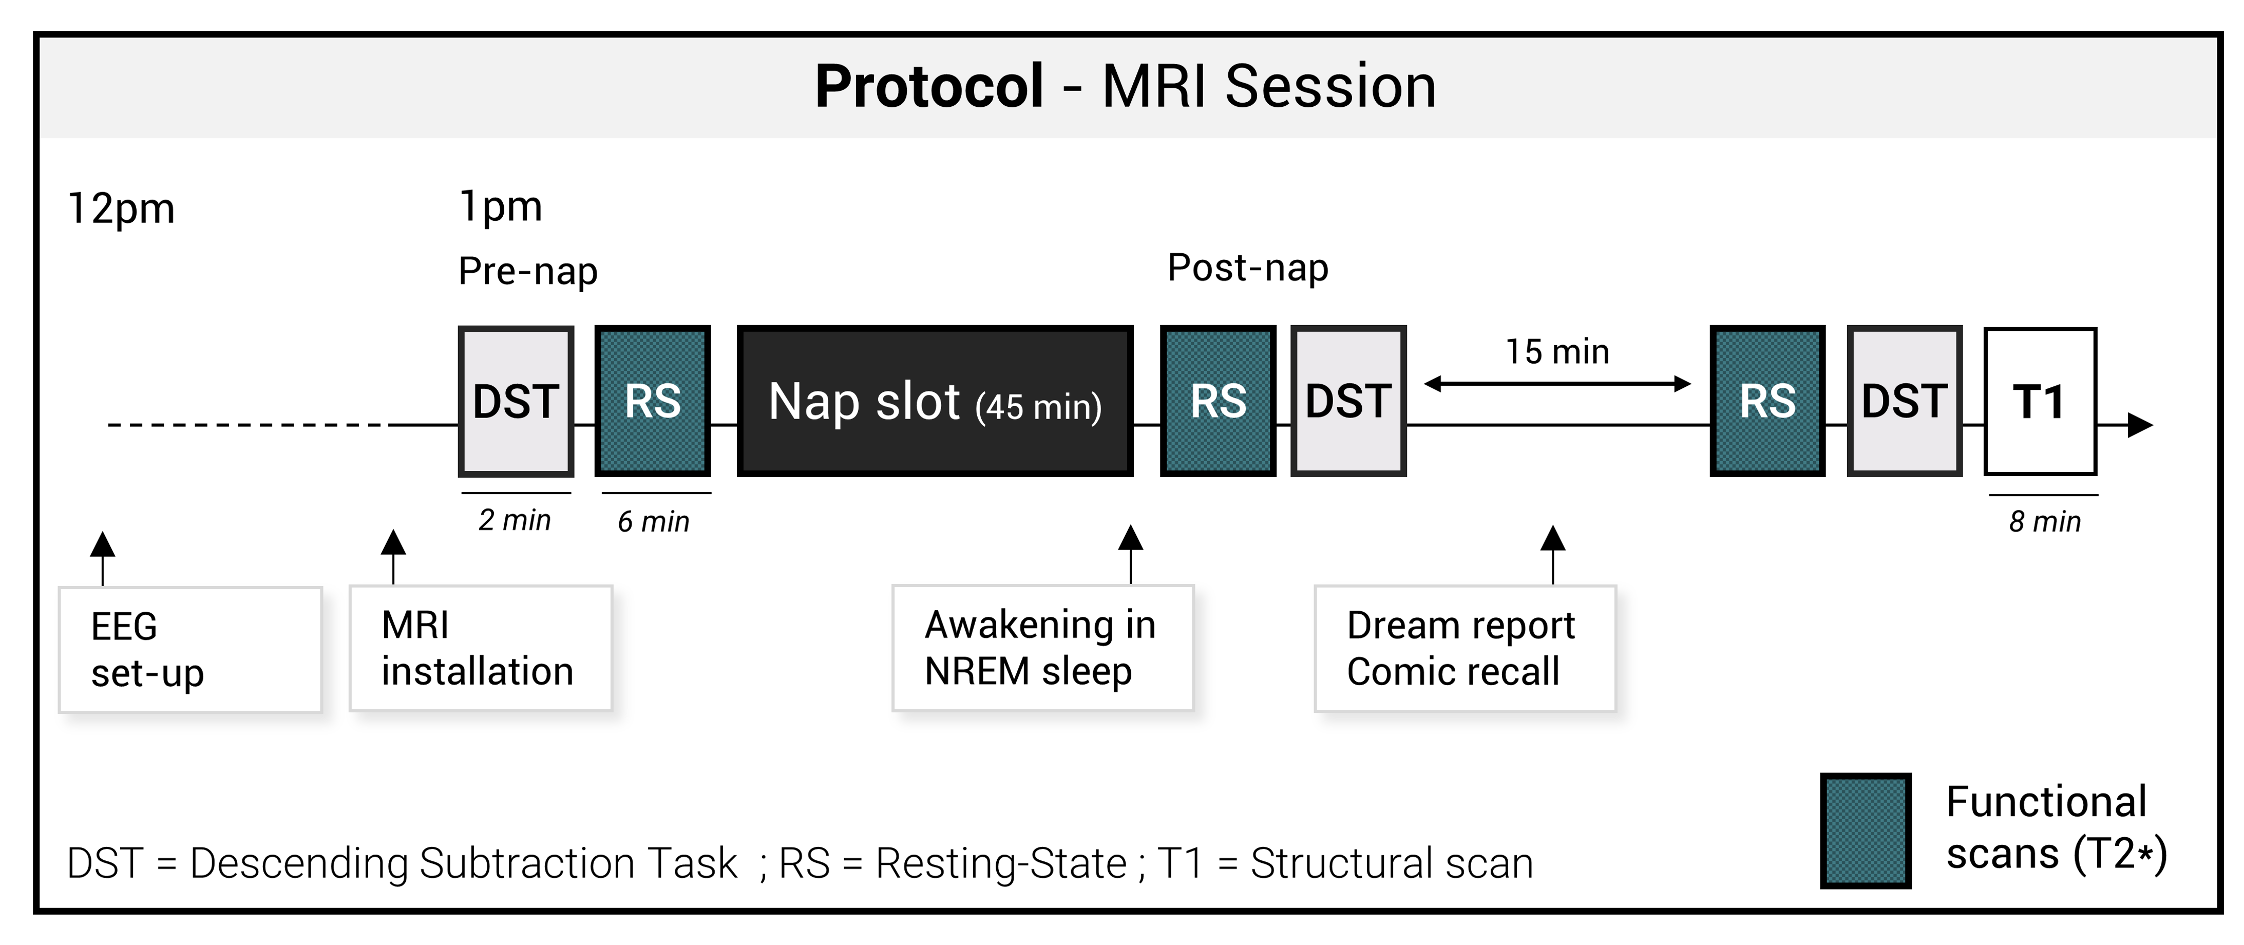
\includegraphics[width=\textwidth]{Fig/Intro/Intro_paradigm_fMRI/Intro_paradigm_fMRI.png}
	\caption[Experimental design of the fMRI study]{\textbf{Experimental design of the sleep inertia fMRI study}. \\
    \emph{\textbf{Participants}}. Participants were selected if they reported and subsequently confirmed during a phone interview having a high or low DRF (DRF superior to 5 dream recalls per week and inferior to 2 dream recalls per month respectively) and having no sleep disturbances. \\
    \emph{\textbf{Evening and night}}. Participants arrived in the sleep unit of the hospital Le Vinatier (Lyon, France) at 8 pm on the evening prior to the experimental day. From 8 pm to 10 pm, they underwent several personality and cognitive tests administered by R.V. They were then instructed to stay awake until 5 am, at which point they were allowed to sleep for 3 hours until 8 am in a bed in the sleep unit. \\
    \emph{\textbf{Day}}. After lunch, participants were conducted to the neuroimaging center (CERMEP). During the first half hour, experimenters installed on the participant’s head a MRI compatible EEG cap. Participants were then installed in the MRI scanner. They read a 5 min comic during the calibration of the eye-tracking camera, and then performed a mental calculation task (descending subtraction task, DST) for 2 minutes. The first resting-state scan was then acquired, with the instructions to remain awake and look at a central fixation cross on the screen. At the end of the scan, participants were informed that they could sleep during the next 45 min. During the nap, the experimenter used the EEG recordings to visually monitor, in real-time, the sleep stages. At the end of the nap slot, participants were awakened, if they were sleeping, by calling their first name and the 2nd resting state scan was acquired. At the end of the scan, the 2nd DST was performed. During the following 10 minutes, subjects were asked about their dream(s) and the comic they had read earlier. Then the 3rd resting state scan and DST were performed (about 25 min after awakening). Finally, an 8-min T1 anatomical scan was acquired.}
	\label{fig:intro:problematics-fmri-paradigm}
\end{figure}

% Using EEG, some studies have found a persistence of slow wave activity in the minutes following awakening, specifically in posterior areas, a phenomenon which has been suggested to represent the electro-physiological signature of sleep inertia \citep{ogilvie_falling_1992, ferrara_electroencephalographic_2006, marzano_recalling_2011, gorgoni_eeg_2015}. Using PET, \citet{balkin_process_2002} reported that the brain areas whose regional cerebral blood flow (rCBF) was increasing between 5 to 20 min post awakening were primarily anterior heteromodal areas (e.g. lateral prefrontal cortices, and anterior insula). They also reported shifts in the relative levels of rCBF between pairs of brain regions (orbitofrontal cortex and ventromedial caudate nucleus, dorsolateral prefrontal cortex and mesencephalic reticular formation) between 5 and 20 min post awakening, leading them to propose that recovery from sleep inertia could hinge on a resumption of normal levels of both rCBF and functional connectivity between brain areas. The latter hypothesis has been tested in two recent resting-state functional magnetic resonance imaging (fMRI) studies which investigated the variations in brain connectivity between pre-sleep wakefulness, nocturnal sleep (without previous sleep deprivation) and post-sleep wakefulness \citep{wu_variations_2012, tsai_local_2014}. Using paired comparisons between pre- and post-sleep wakefulness, they found a decreased connectivity within the sensory-motor network at awakening but no alterations in the default mode network. This altered connectivity within the sensory-motor network is coherent with the poor motor performances observed at awakening but does not explain the impairments observed in other domains (e.g. cognitive tasks such as mental calculation, \citealp{tassi_sleep_2000, trotti_waking_2016}). Yet, some modifications of the default mode network connectivity could be expected at awakening since several neuroimaging studies showed consistent alterations of the default mode network connectivity during sleep, fatigue and/or falling asleep (see \citealp{picchioni_sleep_2013} for a review).

\subsection{Part 2: Sleep inertia in high and low dream recallers}
\label{sec:problematic:inertia:drf}

The second objective of this study was to test the hypothesis of a differential cognitive and brain functioning during the transition from sleep to wake between HR and LR. Indeed, as we have seen earlier (section \ref{sec:dream-recall:theories:inertia})), several studies indicate that sleep inertia could be a critical factor mediating the forgetting or recall of dreams upon awakening \citep{schredl_factors_2003, conduit_poor_2004}, an hypothesis that has however never been experimentally tested. In order to fill this gap, we designed the previously described EEG-fMRI study to study the cognitive and brain functioning upon awakening from sleep, and specifically included in our study participants that were either HR or LR. Our hypothesis was that LR would suffer from more acute sleep inertia upon awakening and that stronger impairment of cognitive functioning would prevent the short term memory of dreams from surviving the sleep-wake transition. Accordingly, we predicted that HR would show (1) more frequent dream recall upon awakening (2) a higher functional connectivity within the default mode network (see section \ref{sec:dream-research:attempts:dmn} and \ref{sec:dream-recall:param:neuro}) (3) less cognitive performance impairments, suggesting a faster recovery from sleep of regions involved in executive and memory processes. In other words, we hypothesized that the brain functional organization during sleep inertia would differ between high and low dream recallers and would reflect between group differences in dream recall.

\section{Study 3. DRF, cognitive abilities, and default mode network}
\label{sec:problematic:dmn-crea}

As we have seen earlier, there is ample evidence that DRF is positively correlated with psychological factors such as creativity or some personality traits (e.g. openness to experience, see section \ref{sec:dream-recall:param:psych} and \ref{sec:dream-recall:param:psych}). On the other hand, recent findings indicate that DRF is also positively associated with distinct neurophysiological traits during both sleep and wakefulness, such as a higher regional cerebral blood flow within core regions of the default mode network. These two observations are remarkably consistent with the emerging view that dreaming and creative-thinking pertain to the same family of spontaneous mental processes, which could be underpinned by a strong recruitment of the default mode network (DMN, \citealp{christoff_mind-wandering_2016}, see section \ref{sec:dream-research:attempts:dmn}) To better delineate the relationship between DRF and the DMN, we re-analyzed the fMRI data of Study 2 to compare, between HR and LR, the functional connectivity of the default mode network, independently of sleep inertia. To this aim, we concatenated the three resting-state scans acquired for each subject, and subsequently compared the global DMN functional connectivity of HR and LR.

Furthermore, we analyzed in this study the numerous cognitive and personality tests that were administered between 8pm and 10pm, on the evening prior to the partial sleep deprivation. Examples of these include the Guildford's Alternate Uses Task \citep{guildford_alternate_1978}, which measures creativity, the Wechsler Memory Scale \citep{wechsler_mem-iii:_2001} to measure memory abilities, and the Big Five Inventory \citep{john_big_1999} which measures an individual on the big five personality dimensions. Regarding the results, we expected that HR would exhibit a higher DMN functional connectivity, specifically between the TPJ and MPFC (see section \ref{sec:dream-recall:param:neuro}), as well as higher scores of creativity and higher scores on certain personality dimensions such as openness to experience. In view of the literature, we did not expect HR to show higher memory abilities than LR.

\FloatBarrier

\section{Study 4. Sleep and dream habits in a sample of French students}
\label{sec:problematic:survey}

Epidemiological investigations in healthy subjects combining questions on both sleep and dreaming are relatively rare. Such measures are yet necessary to establish and keep up to date sleep and dream norms in the general population. Of particular interest is the college population, which is more at risk of suffering from sleep difficulties than the general population \citep{buboltz_sleep_2001, curcio_sleep_2006, forquer_sleep_2008, lund_sleep_2010}.

In order to recruit participants for our above-mentioned fMRI sleep study (section \ref{sec:problematic:inertia}), we have sent an announcement to several mailing lists of students from Lyon University. The announcement comprised a link to an online questionnaire about sleep and dream habits that participants had to fill out. The analysis of the responses provided up-to-date data on sleep and dream habits of a large sample of French college students, pertaining to different academic fields (i.e. humanities, science, medicine). Because our survey included relatively rare questions (e.g. frequency of recurrent and lucid dreams, sleepwalking, sleep-talking, sleep agitation), and thanks to a large sample of students including much more males than in previous studies (i.e. more than one third), we believe that this study will make a significant contribution to the limited number of previous epidemiological studies. Among our main points of interests were (1) to evaluate the sleep patterns of French college students (2) to find whether we could replicate previously reported gender differences in sleep and dream patterns (3) to find whether we could observe some inter academic fields differences.

\section{Study 5. The relationship between waking life and dream content}
\label{sec:problematic:wle}

As we mentioned earlier, there are numerous results showing that waking-life experience (WLE) finds its way into dreams (which led to the so-called continuity hypothesis, \citealp{schredl_continuity_2003}). However, the selection rule and time course of the WLE integration into dreams are still unclear. For instance, few studies have so far investigated the incorporation of WLE from the distant past as well as the incorporation of trivial, mundane, WLE. This is partly due to the classic method used in experimental studies so far, i.e. the content matching paradigm. It requires the participants to rate a posteriori (i.e. at the end of several days of experiment), similarities between a day diary and a dream diary completed for 14 days (e.g. \citealp{schredl_factors_2006, malinowski_evidence_2014}). Such a method has the advantage of controlling for retrospective availability of memories for elements when participants relate dream content to WLEs, but it may have the drawback of missing numerous mundane WLE that are not recorded in the day diary (typically insignificant day-residues), and at the same time overestimating the proportion of emotionally intense WLE. As a consequence, previous studies could not fully assess whether mundane WLEs and/or WLEs from the distant past were incorporated into dreams.

% This is the case for instance regarding the temporal distance between the WLE and its incorporation into dreams on one hand, and the emotional intensity of the WLE on the other hand. Indeed, it is generally admitted that there is a preferential incorporation of recent and emotional WLE into dreams \citep{botman_dream_1990, strauch_dem_2004, grenier_temporal_2005, schredl_factors_2006, malinowski_evidence_2014}. However, some characteristics of dream content do not fit with this modeling of the data. Firstly, some body injuries - be it congenital or acquired - such as amputation, paraplegia and deafness, are less incorporated into dream reports than this model would predict considering how highly emotional and central to the person’s life they are \citep{voss_waking_2011, saurat_walking_2011, bekrater-bodmann_post-amputation_2015}. Secondly, as noticed by \citet{freud_interpretation_1900} more than one century ago, dream content seems to integrate a non-negligible proportion of non-emotional and mundane day residues (i.e. WLEs from the day before the dream).

To address this problem, we designed a study which aimed at investigating in further details the characteristics of the WLEs incorporated into dreams, notably by assessing their remoteness on a life-time scale and by taking mundane WLEs into account. To do so, instead of asking dreamers to keep a day diary, we asked participants to report and characterize the WLEs related to their dreams immediately upon awakening. This strategy presents several advantages regarding previous methods. Firstly, any remembered WLE at any timescale can be considered. This method offers then the possibility of investigating the incorporation of WLEs across the whole life span, which has been rarely attempted until now \citep{grenier_temporal_2005, marquardt_empirical_1996}. Secondly, as the reported memory sources of a dream are dependent on the delay between the dream and the task to report memory sources, the sooner the task after the dream, the more chances we have to identify the true memory sources of the dream \citep{cavallero_dream_1987}. Thirdly, as the connections between elements of waking life and dream content are assessed when the memories of the preceding days are still fresh, this method enables the recall of trivial WLEs from at least the few days before the dream. Using this new approach, we were able to test whether emotional WLEs are still preferentially incorporated into dream reports when trivial WLEs are taken into account and to investigate the emotionality and significance of WLEs incorporated into dreams as a function of their remoteness.

We predicted that this methodology would enable us to observe that a large proportion of the WLEs incorporated into dreams are mundane. Regarding the temporal remoteness of the WLEs incorporated into dreams, we expected to find not only a large contribution of the day before the dream \citep{marquardt_empirical_1996} but also a significant contribution of remote WLEs \citep{verdone_temporal_1965, grenier_temporal_2005, llewellyn_such_2013}. Finally, given previous results showing a tendency for dreams to incorporate preferentially emotional WLEs \citep{schredl_factors_2006, malinowski_evidence_2014}, and the claim that day residues are predominantly mundane \citep{freud_interpretation_1900}, we predicted an interaction between remoteness and emotionality for WLEs incorporated into dreams. Specifically, we expected that day residues would be scored as less important and less emotionally intense than would be more remote WLEs incorporated into dreams.

\section{Study 6. An open-source software for sleep reading and analysis}
\label{sec:problematic:software}

During my PhD thesis, I have been working extensively on polysomnographic sleep recordings, notably to score sleep microstructural events (e.g. arousals, rapid eye movements; see section \ref{sec:problematic:arousals}) and sleep stages (see section \ref{sec:problematic:inertia}). While the detection of sleep microstructural events is usually done with automatic algorithms, the identification of sleep stages is traditionally done visually by an expert. For both visual sleep staging and automatic microstructural analysis, sleep researchers use either commercial or in-house softwares. In many cases, these softwares come with their own data and hypnogram file formats, and this heterogeneity can represent a substantial obstacle for sharing of algorithms and sleep data across laboratories.

% Some of the very few free and open-sources alternatives allowing scoring and to some extent analysis of sleep data are \fnurl{Phypno}{https://pypi.python.org/pypi/phypno} and \fnurl{SpiSOP}{http://www.spisop.org/}, yet they do not include graphical integration of automatic detection and are largely based on command-line options, which are hardly accessible for users with little or no programming knowledge.

% Traditionally, the scoring of sleep micro- and macro-structure is done visually and requires therefore a considerable investment of time and effort, in addition with being subject to both inter and intra-rater variability. Sleep scoring can also be done using automatic methods which have the advantage of being fast, reproducible and with generally good agreement with visual scoring \citep{berthomier_automatic_2007, lajnef_learning_2015}. Yet automatic scoring is far from being widespread and most sleep laboratories still rely on visual scoring, using either commercial softwares or in-house packages. In many cases, these softwares come with their own data and hypnogram file formats, and this heterogeneity can represent a substantial obstacle for sharing of algorithms and sleep data across laboratories or clinics. Some of the very few existing and up-to-date open sources alternatives allowing reading and scoring of sleep data are \fnurl{Phypno}{https://pypi.python.org/pypi/phypno} and \fnurl{SpiSOP}{http://www.spisop.org/}, yet they do not include graphical integration of automatic detection and are largely based on command-line options, which are hardly accessible for users with little or no programming knowledge.

In view of this, I developed, during my PhD thesis, a free and open-source software capable of reading numerous file formats, and integrating several signal processing tools and automatic detection of sleep microstructure. At first intended for my personal use, it soon extended into a fully developed and comprehensive software, thanks to a collaboration with my fellow PhD student \fnurl{Etienne Combrisson}{https://etiennecmb.github.io/}. This software was integrated into a broader neuroscientific suite named \fnurl{Visbrain}{http://visbrain.org/}, and the specific sleep module was named \textit{SLEEP}. The primary aim of \textit{SLEEP} is to provide a fast and intuitive graphical user interface (GUI) to visualize and score polysomnographic sleep recordings. In order to be widely disseminated, the software must support a large range of data file formats, both proprietary (e.g. BrainVision) and public (e.g. European Data Format). It should also be able to handle the great heterogeneity in hypnogram formats (e.g. sampling rate of the hypnogram, values assigned to each sleep stage). Finally, to provide a significant scoring aid, the software should include several automatic detection algorithms (e.g. spindles, K-complexes, slow-waves) and several signal processing tools (e.g. filtering, referencing). Altogether, we believe that this software could represent a major methodological development in the field of sleep research.

\section{Summary}
\label{sec:problematic:summary}

\begin{figure}[htb]
	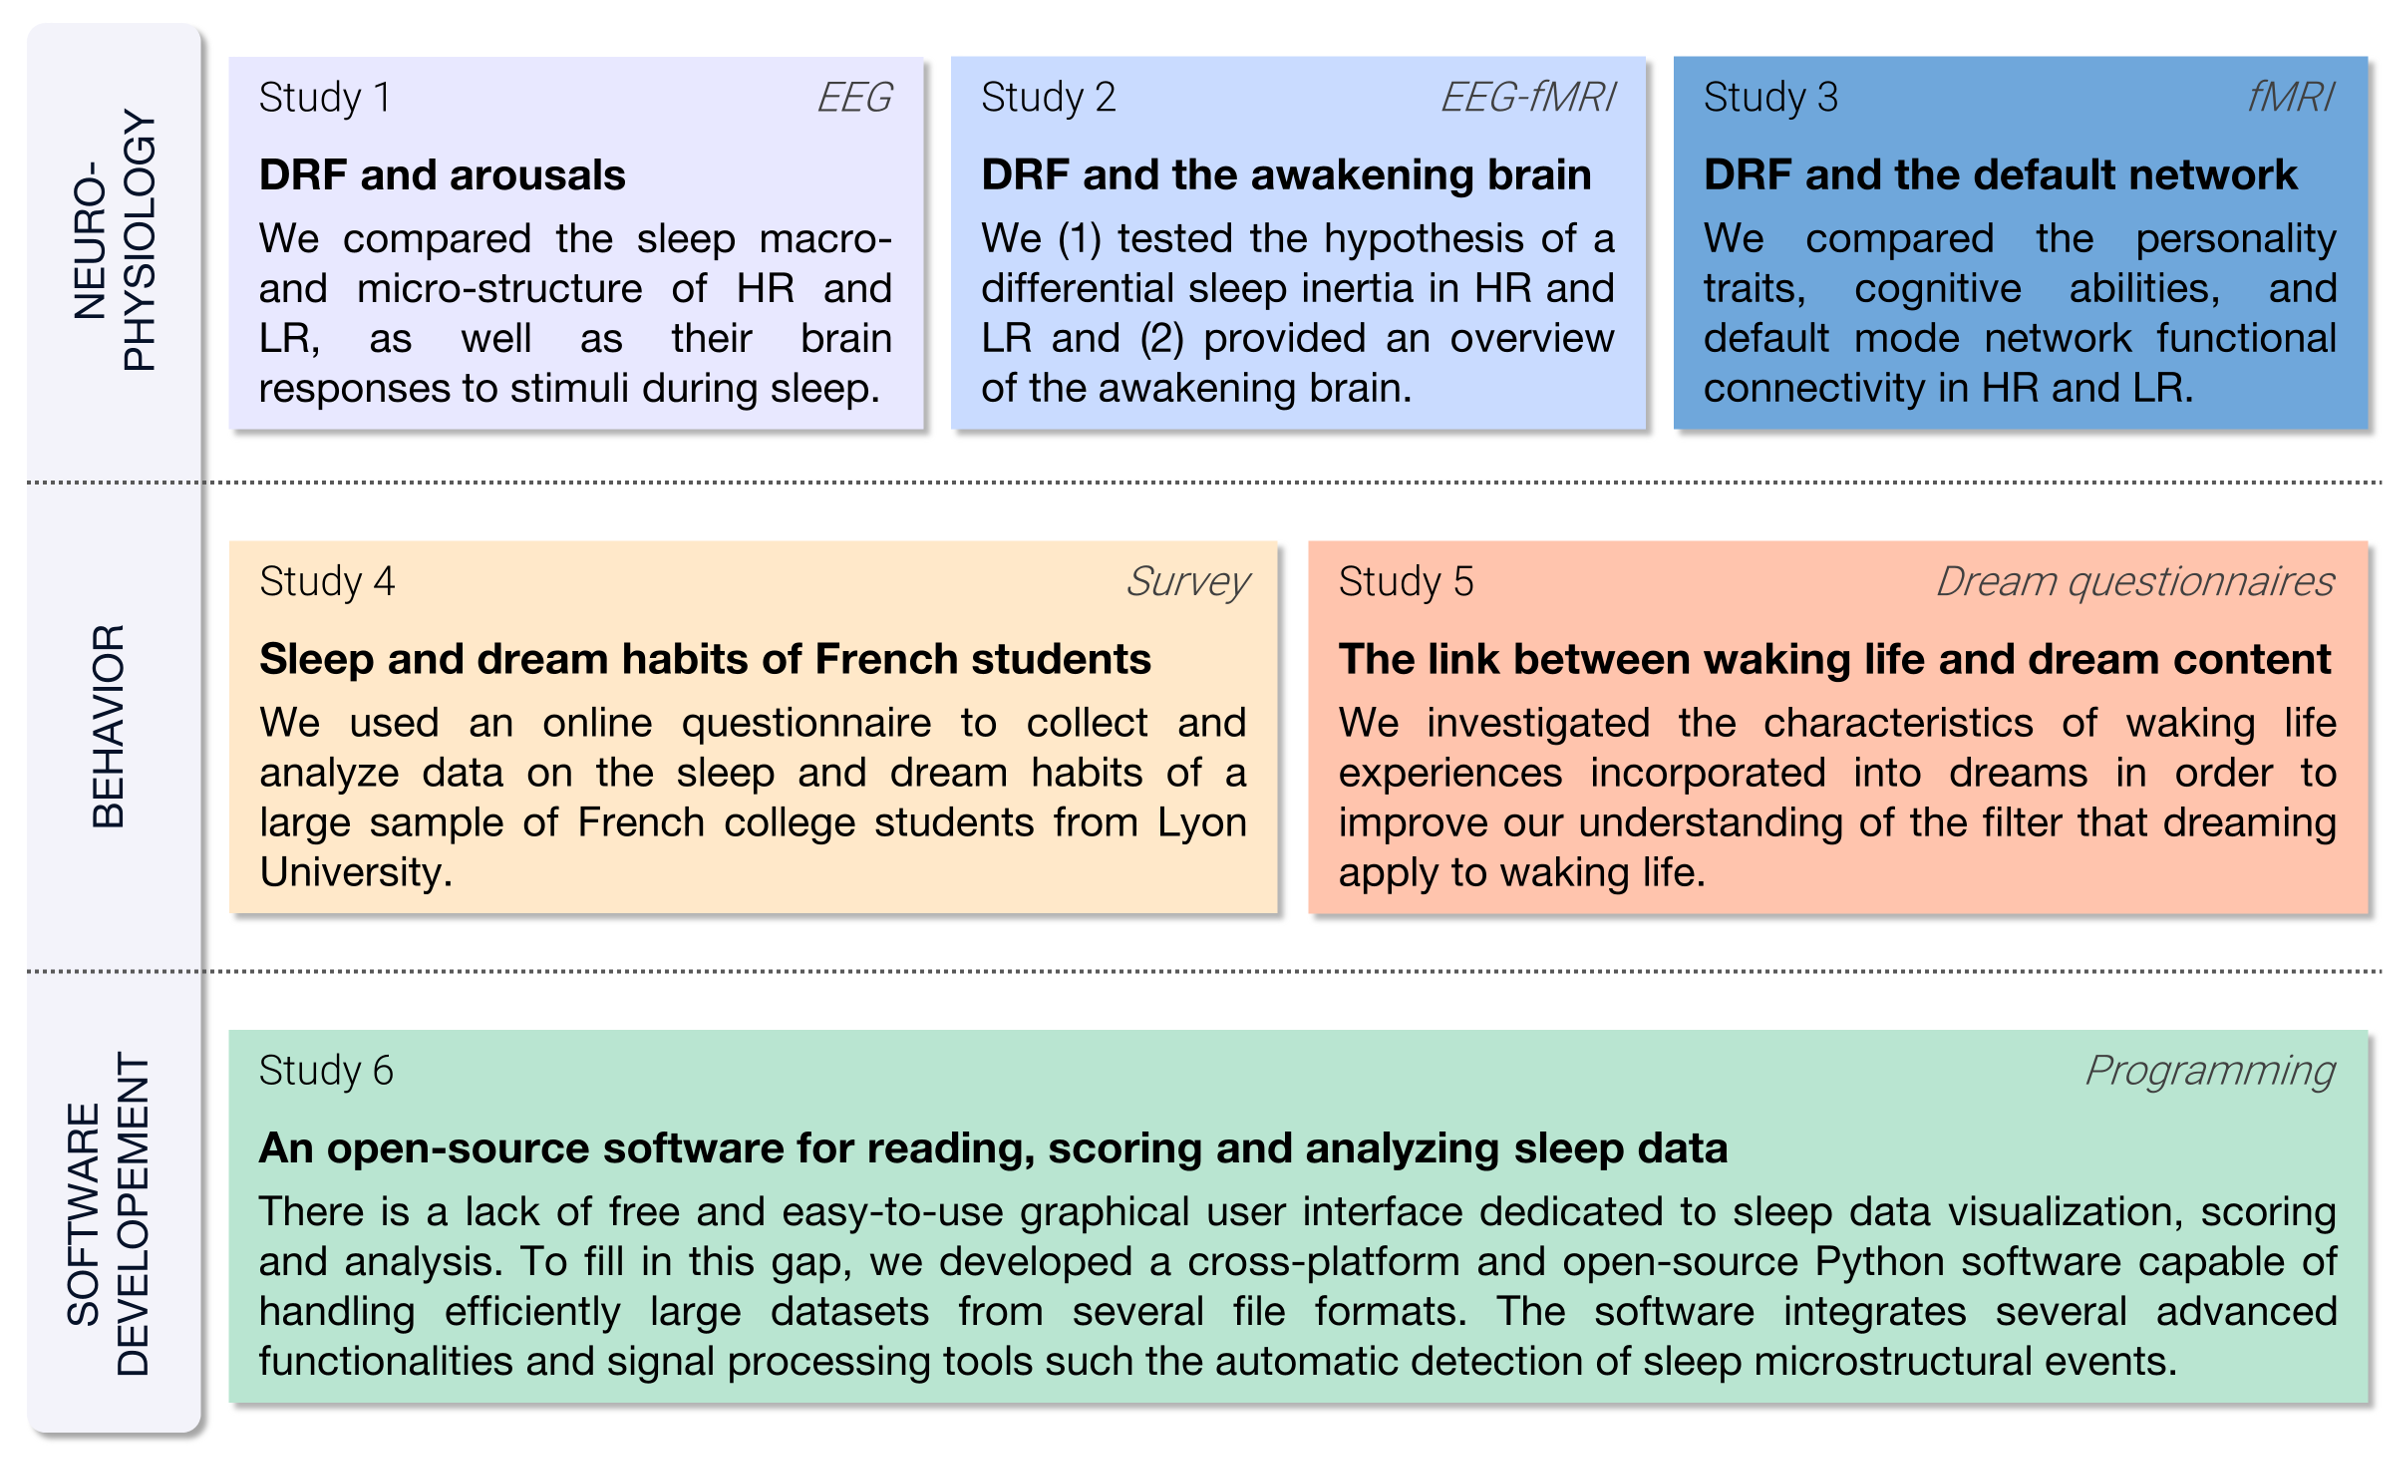
\includegraphics[width=\textwidth]{Fig/Intro/Intro_Problematics/Intro_Problematics.png}
	\caption[Summary of the studies conducted during my PhD thesis]{\textbf{Summary of the studies conducted during my PhD thesis}. In Studies 1, 2 and 3, we investigated the neurophysiological correlates of dream recall frequency (DRF), by comparing the sleep parameters, cognitive abilities and brain functional connectivity of high and low dream recallers (HR and LR respectively). Second, we used behavioral methods to collect data on the sleep and dream habits of college students (Study 4), as well as the relationship between waking life and dream content (Study 5). Finally, Study 6 relates to the ongoing development of an open-source software dedicated to sleep data.}
	\label{fig:intro:problematics-summary}
\end{figure}
